\documentclass{beamer}
\usepackage{graphicx}
\usepackage{amsmath}
\usepackage{listings}
\lstset{language=html}
\usepackage{array}
\usepackage{biblatex}
\addbibresource{rapport.bib}
\usepackage{hyperref}
\graphicspath{{~/templates/}, {../images/}}
\usetheme{Hannover}

\addtobeamertemplate{navigation symbols}{}{%
	\usebeamerfont{footline}%
	\usebeamercolor[fg]{footline}%
	\hspace{1em}%
	\insertframenumber/\inserttotalframenumber
}


\begin{document}
	
	\title{Mémoire de stage}
	\maketitle
	
	\begin{frame}
		
		\tableofcontents
		
	\end{frame}

	\section{Contexte du stage}
	\subsection{Inria}
	\begin{frame}
		\frametitle{L'Inria}
		\centering
		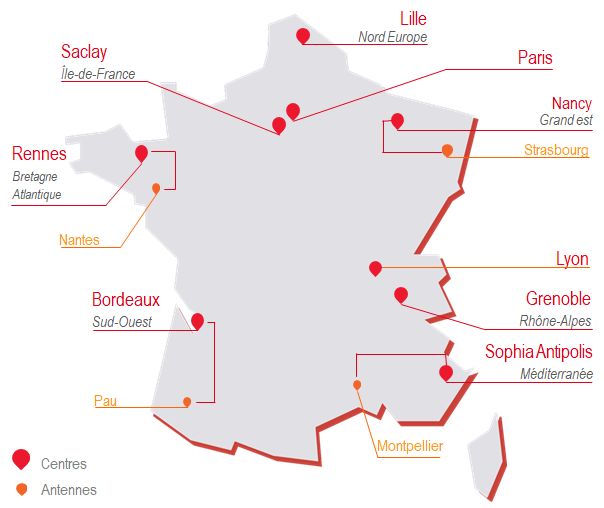
\includegraphics[width=0.4\textwidth]{cartecentres.png}
		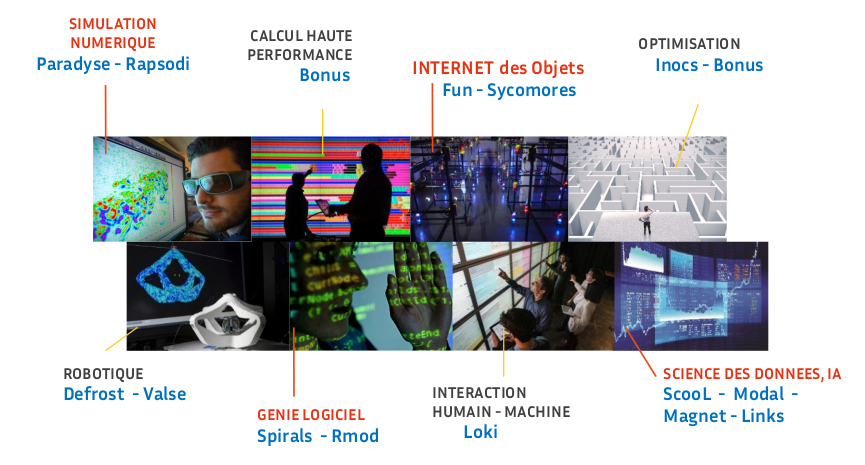
\includegraphics[width=0.8\textwidth]{equipesCentre.png}
	\end{frame}

	\subsection{Le projet AmIUnique}
	\begin{frame}
		
	\end{frame}

	\begin{frame}
		
		\printbibliography
		
	\end{frame}
	
\end{document}